\documentclass{article}
\usepackage[numbers]{natbib}
\usepackage{amsmath}
\usepackage[ruled,linesnumbered]{algorithm2e}	
\usepackage{multirow}
\usepackage{hyperref}
\usepackage{float}
\usepackage{xcolor}
\usepackage{graphicx}
\usepackage{booktabs}
\usepackage{caption}
\usepackage{array}
\hypersetup{
	colorlinks,
	linkcolor=blue,
	filecolor = blue,
	citecolor=red,
	urlcolor=blue
}\setlength{\belowcaptionskip}{-15.0pt}
\title{Implementation and Empirical Comparison of Gradient-Descent-Based Optimizers}
\author{Kenan Karavoussanos}
\begin{document}


\pagenumbering{roman}
\maketitle
\begin{abstract}	
	
	The choice of Optimizer for an Artificial Neural Networks requires multiple considerations, including length of training time, reliance on initial training constants and ability to converge to a global minimum rather than a local minimum. This paper presents and compares Gradient-Descent-Based Optimizers. These Optimizers are compared in the context of an Artificial Neural Network classifier on the MNIST dataset of handwritten digits using Loss and Accuracy as comparison metrics. It was shown that the use of momentum and cyclical learning rates provide better performance than vanilla gradient descent, with momentum providing a larger improvement.The tested adaptive learning rate optimizers, ADAGRAD,RMSProp and Adam performed better than vanilla gradient descent, momentum, cyclical learning rates and search-then-converge. The Search-Then-Converge learning rate schedule reduced the performance vanilla gradient descent. This comparison is not universally applicable due to the stochastic nature of different datasets and problems. The results contained within this report are specifically applicable to Multiclass classification problems.
\end{abstract}	
\thispagestyle{empty}
\newpage
\clearpage
\setcounter{page}{1}
\tableofcontents
\newpage
\section*{Symbols and Nomenclature}
The following section contains definitions and elaborations on important, domain-specific, terms and acronyms. This section serves as an aid and reference to the reader of this report.

\subsection*{Nomenclature}
\begin{itemize}
	\item Artificial Neural Network: A massively distributed and parallelized processor made up of small computational units called Neurons that acquires knowledge from its environment through a learning process and stores this knowledge as synaptic weights between neurons ~\cite{ANNDefinition}.
	\item Multi-Layer Feed-Forward Network: An Artificial Neural Network where the neurons are arranged in distinct layers. Where input flows unidirectionally from the input layers to the output layer with no feedback to previous layers. Also referred to as a Multi-Layer Perceptron Network.  
	\item Loss Function: A function that is used to evaluate the error in an Artificial Neural Network. 
	\item Optimizer: A function that attempts to minimize the Loss Function i.e the error of an Artificial Neural Network by changing the values of the weights in the network.
	\item Gradient Descent: An Optimizer that uses the gradient of the Loss Function when minimizing.
	\item Learning/Training Process: The process of reading inputs, calculating the error and minimizing said error in an Artificial Neural Network. 
	\item Learning Rate: The size of the updates an Optimizer makes to the weights of a Network during the Training Process.
	\item Generalization: The ability of a Neural Network to perform its learning task i.e classification on data it did not see during the learning process. 
	\item Overfitting: The state of a Network where it fits to the training data too well resulting in poor generalization.
	\item Epoch: A single pass over the set of training inputs in the Training Process.
	\item Hyperparameter: A parameter of an Artificial Neural Network set before the start of the Training Process.
	\item Regularization: A hyperparameter that introduces a penalty for relying too heavily on a specific Neuron in the Network. This prevents the network from overfitting to the training data.
	\item Dropout: The act of temporarily removing a specific Neuron in a Neural Network during the Training Process to prevent the Network from relying too heavily on said Neuron. This also refers to a hyperparameter that determines the probability of Dropout occurring for a specific neuron. 
	\item Accuracy: The proportion of correctly classified inputs made by an Artificial Neural Network to the total number of tested inputs.
	\item MNIST Dataset: A dataset of 28x28 pixel handwritten digits from 0 to 9.
	\item Gradient Acceleration Method: A general class of improvement to optimizers that involves keeping the optimizer moving along the trend in the gradient as opposed to following smaller, local changes in gradient.
\end{itemize}
\subsection*{Symbols}
\begin{itemize}
	\item ANN: Artificial Neural Network
	\item MLP: Multi-Layer Perceptron Network
	\item SGD: Stochastic Gradient Descent
	\item STC: Search-then-Converge
	\item CLR: Cyclical Learning Rate
	\item RMS: Root Mean Squared
	\item ReLU: Rectified Linear Unit
\end{itemize}
	
\newpage
\listoffigures
\listoftables

\newpage
\pagenumbering{arabic}
\section{Introduction}
\subsection{Artificial Neural Network} 
\begin{figure}[h]
	
	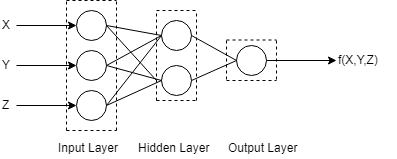
\includegraphics[width=\textwidth,keepaspectratio]{ANN_Diagram.png}
	\setlength{\belowcaptionskip}{0.0pt}
	\caption{Diagram of an ANN}
	\setlength{\belowcaptionskip}{-15.0pt}
\end{figure}
\paragraph{}An Artificial Neural Network(ANN) is defined as a massively distributed and parallelized processor made up of small computational units called Neurons that acquires knowledge from its environment through a learning process and stores this knowledge as synaptic weights between neurons ~\cite{ANNDefinition}. A Neuron, pictured as a circle in Figure 1, takes external data or data from other neurons as input via synapses, pictured as the lines between neurons, coming in and out of it. Each input is multiplied by its respective synaptic weight, which is a value representing the strength of the synaptic connection, and then this weighted sum is passed through a function called an activation function to produce a single value called the activation. This activation acts as input to the next layers of Neurons until the Network produces an output.

The learning process is typically modeled by the backpropogation algorithm combined with an update rule. The backpropogation algorithm is responsible for assigning blame for error in the network's output to the neurons of the network. Once this blame has been assigned, the update rule i.e The Optimizer updates the synaptic weights of each neuron in an attempt to minimize the error function.
\subsection{Architecture}
\paragraph{}Neurons are arranged in layers:
\begin{itemize}
	\item An input layer
	\item An output layer
	\item Zero or more hidden layers. So called as the inputs and outputs to and from the neurons in these layers are typically unobserved.
\end{itemize}
In a feed-forward network, output is passed sequentially to the next layer of neurons. The weights between layers are stored in a Weight-Matrix.

\subsubsection{Input Layer}
The Architecture of our ANN will be a Multilayer Feed Forward Network with 2 hidden layers.
It has been proven that a Neural Network with two hidden layers can approximate any bounded continuous function to arbitrary accuracy \cite{Hornik1989}. The data takes the form of 28x28 pixel images. With each pixel being an individual input we have, $\boldsymbol{N}_i$, the number of inputs equal to 784.

\subsubsection{Hidden Layers}

\citet{panchal2014review} suggest a simple approach to selecting the number of neurons in a network by providing some rules of thumb. Specifically,
\begin{enumerate}
	\item	$\boldsymbol{N}_h\in[\boldsymbol{N}_o, \boldsymbol{N}_i]$
	
	\item$\boldsymbol{N}_h < 2\times\boldsymbol{N}_i$
	
	\item$\boldsymbol{N}_h = \frac{2}{3}\boldsymbol{N}_i + \boldsymbol{N}_o$
\end{enumerate}

Following these guidelines as well as the results in ~\cite{deepsimpleMLP} the following architecture has been proposed:

\begin{equation}
\boldsymbol{N}_{h1} = \boldsymbol{N}_{h2} = 300
\end{equation}
so \begin{equation}
\boldsymbol{N}_h = \boldsymbol{N}_{h1} + \boldsymbol{N}_{h2} = 600
\end{equation}



\subsection{Activation Functions}
Activations functions take in the weighted sum of inputs to a neuron and produce the output of the Neuron. These activation functions are typically non-linear.

The hidden layers of the Network used in experimentation made use of the ReLU activation function and the output layer makes use of the Softmax activation function.

The ReLU activation function is given by the following equation:
\begin{equation}
g(z) = \begin{cases} 
z & z > 0 \\
0 & elsewhere
\end{cases}
\end{equation}

The Softmax activation function is given by the following equation:
\begin{equation}
\sigma(\boldsymbol{z})_j = \frac{e^{z_j}}{\sum_{k=1}^{K} e^{z_{k}}} \;\;\; \mbox{for} \;\;\; j = 1, ... , K 
\end{equation}
Where $K$ is the number of classes in the dataset.


\subsection{Loss Function}
A function that describes the amount of error in an ANN. This is the function which is minimized by the Optimizer during the Training Process.

The loss function used in the Network used for this experimentation is the categorical cross-entropy function which is given by:
\begin{equation}
L(\hat{\boldsymbol{y}},\boldsymbol{y}) = -\frac{1}{N}\sum_{i=1}^{N} [y_{i}\log{\hat{y_{i}}} + (1-y_{i})\log{(1 - \hat{y_{i}})}]
\end{equation}
Where $\hat{\boldsymbol{y}}$ is the set of $N$ guessed class labels and $\boldsymbol{y}$ is the set of $N$ actual class labels.
\subsection{Gradient Descent}
Gradient Descent is classified as a first-order iterative optimization algorithm. It works by exploiting the principle that given a multivariable function $J(\underline\theta)$, that is differentiable at a point $\underline{a}$, then $J(\underline\theta)$ decreases fastest along the direction of the negative gradient of $J(\underline\theta)$ at $a$ i.e $-\nabla{J(\underline{a})}$

Given a weight matrix $\underline\Theta$, the gradient descent update rule for the weight $\theta_{ji}$ is given by:
\begin{equation}
\theta_ji \leftarrow \theta_{ji} + \Delta\theta_{ji}
\end{equation}

where the weight update, $\Delta\theta_{ji}$, is given by:
\begin{equation}
\Delta\theta_{ji} := -\alpha\frac{\partial{J}(\theta)}{\partial{\theta_{ji}}}
\end{equation}


$\alpha$ is the learning rate and $\frac{\partial{J}(\theta)}{\partial{\theta_{ji}}}$ is the gradient of the error function with respect to $\theta_{ji}$.
$\frac{\partial{J}(\theta)}{\partial{\theta_{ji}}}$ is calculated using the backpropagation algorithm ~\cite{backpropagationOriginal}.


\subsection{Learning Rate}
The Learning Rate of an ANN can be defined as the rate at which parameters change in a network. That is, given a new update on $\theta_{ji}$, the proportion of $-\frac{\partial{J}(\theta)}{\partial{\theta_{ji}}}$ that is added to the current $\theta_{ji}$ is given by, $\alpha$, our learning rate.
\hfill\newline

The value of the Learning Rate is crucial to the convergence of the network. Too low of a learning rate and the time to convergence becomes exceedingly high. Too high of a learning rate and the network may fail to converge due to continually stepping over the minimum. The Learning Rate can be global to all weights in the network or local to individual or groups of weights. Additionally, the learning rate can be static for the entire learning process or can be adaptive throughout the learning process.


\subsection{The role of an Optimizer in an Artificial Neural Network}	The purpose of an Optimizer in the context of Artificial Neural Networks is to minimize the Loss Function describing the classification error of the ANN. 
	Stochastic Gradient Descent forms the base for many cutting edge Optimizers used in Artificial Neural Networks. This paper provides an overview of the theory behind each Optimizer and compare the Accuracy and Loss of the network once it has gone through the Learning Process.   


	Due to the large amount of computation and calculation required to train an ANN, it is infeasible to trace the training algorithm for more than a few training examples. As such the Loss and Accuracy are used to evaluate the performance of the ANN and its Optimizer. Slow optimizers become prohibitive to training for large datasets so the training "speed" has been chosen as a comparison metric. This training speed shall be measured by comparing the training loss and training accuracy with respect to the number of training examples seen during the learning process. The level of generalization of the network i.e the ability of the network to classify unseen data is the most significant consideration when evaluation the performance of an ANN. Thus the final accuracy and loss over the test set i.e Test Accuracy and Test Loss have also been chosen as comparison metrics for the tested Optimizers. 
	
	\subsection{Significance of problem}
	The current body of research shows evaluations of each Optimizer and how it overcomes specific limitations. However, these evaluations are mainly done in isolation of one another or in comparison with a narrow selection of popular Optimizers. This paper seeks to combine these various isolated evaluations and perform a broad, integrated comparison of each Optimizer
	
	For specific or niche problem domains and datasets, comparing each optimizer allows for the reader to select an appropriate Optimizer to fit within various real world constraints.
	
	The evaluation of each optimizer on the standard MNIST Dataset allows for empirical validation of previous theoretical study on Gradient Descent based Optimizers along our metrics. Due to the generality provided by evaluation on the standard MNIST Dataset, the problem solution is applicable across many domains. However, this generality also makes the comparison less applicable on niche datasets.
	
	
	\subsection{Organization of the rest of the paper}
	
	Section 2 of this paper contains a review of the current body of literature pertaining to the problem described above. Section 3 contains a description of the methodology used when performing the experimentation as well as detailed descriptions of concepts that were espoused in the paper. Section 4 contains derivations for a number of vectorized equations discussed in section 3. Section 5 discusses the experimental and computational setup used in this paper. Section 6 presents graphs and tables of the results obtained during experimentation. Finally, section 7 analyses the results of the experimentation.
	
	
\section{Literature Survey}	
 The following literature review seeks to critically evaluate the current evaluations of various prolific optimizers used in Artificial Neural Networks. In particular, the performance of each optimizer in comparison to others as well as the discussed trade-offs of the optimizer. The speed of training i.e the rate of increase of Training Accuracy and Loss as well as the level of generalization i.e the Test Accuracy and Loss will be focused upon in this review.
 
 
 \paragraph{}~\citet{kingma2014adam} provides an unbiased empirical evaluation of the Adam Optimizer with respect to other optimizers. Adam can be described as a combination of RMSProp, Momentum and a bias-correction term.
 Multiple statistics are used for the comparison and shows that Adam is faster to converge than all the other tested optimizers, however it is admitted that Adam tends to over-fit to the training data so regularization and dropout strategies were used to improve generalization. For a Multi-layer Neural Network with dropout stochastic regularization, the training cost versus iteration number is reported for multiple Optimizers. However, the generalization of these optimizers, along our chosen metrics is not reported.
 
 \paragraph{}~\citet{ruder2016overview} provides an overview of various gradient based optimizers and their specific limitations. However the overview is wholly theoretical and does not report any empirical statistics in its analysis.
 Provided derivations of each optimizer have been used in the current work for the development of the algorithms used in each  A visualization of some of the discussed optimizers is provided but this does not specifically pertain to the domain of our problem as the visualized objective functions are geometric functions as opposed to Loss functions. It is important to note the poor performance around saddle points of the optimizers with static learning rates.
 
 
 \paragraph{}~\citet{darken1991note} discusses learning rate schedules as a solution to a static learning rate as well as introduces the Search-Then-Converge (STC) Method. A major limitation to learning rate schedules discussed is that the learning rate decreases too quickly so convergence is not guaranteed. STC attempts to solve this problem by slowing down this reduction in learning rate and then increasing the reduction once a certain time threshold has been reached. This gives the optimizer time to \textit{search} for a local minimum and then \textit{converge}, hopefully, once it is found. The paper describes that this method is \textit{guaranteed} to converge, however there is no proven guarantee that the optimizer will find a local minimum within the "search" period. This bias warrants that further investigation be reported in the current work to validate the claims of this paper.
 
 \paragraph{}~\citet{duchi2011adaptive} proposes the Adaptive Subgradient Method ,or ADAGRAD.The performance of this method is gauged along two metrics. The online error as well as the test set performance of the resultant classifier after one learning epoch. Various other adaptive gradient methods are tested for comparison and it is shown that ADAGRAD is the best optimizer to use when the training dataset is sparse i.e the set is too small to fully describe the trend in the data. However, for small datasets, ADAGRAD is beat by the AROW algorithm. It is also shown that, on MNIST classification, the error rate for ADAGRAD is 0.4\% greater than that of the Passive-Aggressive Algorithm. The version of ADAGRAD tested in this paper involves the use of Regularised Dual Averaging, which is a form of weighted average and thus differs from the ADAGRAD version to be tested in the current work.
 
 \paragraph{}~\citet{smith2017cyclical} proposes  the use of cyclical learning rates as opposed to adaptive learning rates. Cyclical learning rates (CLR) are shown to have less computational cost than other adaptive methods.  The accuracy at 25000 and 70000 training iterations is used as a comparison metric for the different optimizers tested.
 The method involves sampling a periodic function which is bounded by a maximum and minimum learning rate. This prevents the learning rate from monotonically decreasing as in ADAGRAD or other learning rate scheduling techniques. This improves the performance of the optimizer around saddle points. Selecting a minimum and maximum learning rate as well as the cycle length of the periodic function is covered by a selection of tests contained within the paper. 
 
 \paragraph{}An interesting result in the paper shows that when using CLR with a gradient acceleration method, The Nesterov Method, it took only 25000 training iterations to achieve accuracy similar to the regular Nesterov Method after 70000 iterations. Similarly, RMSProp with CLR achieves the same improvement. However, when CLR is used in conjunction with the Adam Optimizer, the performance is worse than the regular Adam Optimizer. This suggests some conflict with CLR and either the first-moment term, the bias correction or both in the Adam Optimizer.
 
 \paragraph{}~\citet{Simard2003BestPF} describes the best practices for Convolutional Neural Networks. In particular using elastic deformation to increase the number of training examples is suggested as a standard for CNN training. It is shown that elastic deformation produces better generalization of the network when compared to affine deformation which in turn is better than no deformation. These methods may potentially be used if the network overfits the training data. This is a computationally expensive method to prevent overfitting when compared to regularization or dropout methods. However, the distortion can be precomputed and reused for various experiments which could potentially save computation time across all experiments in this work. Although this article describes best practices for CNN's this best practice applies to our domain as the dataset is the same.
 
 \paragraph{} ~\citet{lecun1998gradient} compares various types of classifiers on the MNIST database. A MLP with one hidden layer achieved a $4.7\%$ test error with 300 hidden units and $4.5\%$ for a network with 1000 hidden units. This marginal improvement for a large increase in hidden units suggests that the network with 1000 units was overfit i.e poorly generalized, thus the increase in units past a certain threshold between 300 and 1000 increases test error. Alternatively, the increase in number of hidden units could follow a law of diminishing returns and thus while adding units does not increase test error, doing so may not strictly decrease test error. Irrespective of which case holds, it can be seen that arbitrarily adding hidden units does not significantly improve test error and thus other guidelines such as computational time should be considered when deciding on network architecture. A similar pattern holds for a network with two hidden layers.
 
 \paragraph{}~\citet{deepsimpleMLP} evaluate the effect of the number of layers and number of neurons per layer in a Multilayer Perceptron(MLP) Artificial Neural Network when classifying Handwritten Digits. Training examples were distorted using elastic and affine deformations. This distortion was used to artificially increase the number of training examples by distorting all training images in each training epoch. GPU acceleration was used to reduce the training time for each network. The performance of each architecture was measured primarily via the minimum test error achieved at each training epoch. While trialling various architectures the best minimum test error was achieved by a network with 5 hidden layers with 2500,2000,1500,1000,500,10-architecture at $0.32\%$ error. However the training time required to achieve this result was 114.5 hours. A two layer MLP with 1000,500,10-architecture achieved $0.44\%$ error on the test set while only taking 23.4 hours of training time. 
 
 
 

  
\section{Methodology}


  


\subsection{Dataset}

The Dataset the ANN will be trained on is the MNIST training set. It is a dataset of 60000 28x28 pixel images of handwritten decimal digits  from 0 to 9. In total there are 10 distinct classes of images. The classes are evenly distributed thus the dataset is considered balanced.

The Dataset the ANN will be tested on is the MNIST test set. It is similar to the above training set however there are only 10000 images.

\subsection{Performance Metrics}
This section describes the manner in which the various Optimizers are compared and evaluated.
\hfill\newline
During training on a given Optimizer, the Training Accuracy and Loss were sampled after every 100 training examples. The Test Accuracy and Loss were sampled every 6000 examples. These four metrics were all averaged over 10 training process instances. 

The training metrics serve as a temporal plot of the network learning speed while the test metrics serve as a temporal plot of the generalization of the network.

Stochastic Gradient Descent serves as our control for comparison for the other Optimizers.
\subsection{Momentum}
The Momentum Method is an acceleration method \cite{backpropagationOriginal} used to overcome sudden changes in gradient, that are common around minima, and reduce the time to convergence by setting the next weight update equal to a linear combination of:
\begin{enumerate}
	\item $\frac{\partial{J}(\theta)}{\partial{\theta_{ji}}}$ the gradient of the error function with respect to $\theta_{ji}$
	\item $\Delta\theta_{ji}$ the previous weight update.
\end{enumerate}  
\begin{equation}
\Delta\theta_{ji_{t+1}} := -\alpha\frac{\partial{J}(\theta)}{\partial{\theta_{ji}}} + \beta\Delta\theta_{ji}
\end{equation}


\hfill \newline
Where $\beta<1$ is the momentum, or exponential decay, constant 
\hfill \newline

Doing this improves the ability of the optimizer to avoid local minima by allowing it to follow the overall trend in gradient rather than the instantaneous gradient. This also speeds up convergence as once the trend in the gradient is found, the optimizer accelerates along this trend towards the minimum.
\hfill\newpage
\subsection{Learning Process Algorithms}


\subsubsection{Learning Process With SGD}
The algorithm below shows the full learning process involving the backpropagation algorithm and the SGD optimizer.
\begin{algorithm}[h]
	\SetAlgoLined
	\KwIn{Training Symbols  $\{(\underline{x}_0,\underline{y}_0), ... , (\underline{x}_n,\underline{y}_n)\}$ }
	\KwOut{Weight Matrices $\boldsymbol{\Theta}$}
	
	Initialize all weights in all weight matrices $\boldsymbol\Theta^{(l)}$ to small non-zero gaussian random numbers.
	
	Initialize all update matrices $\boldsymbol{\Delta\theta}^{(l)}$ to zero matrices.
	
	\ForEach{ $(\underline{\boldsymbol{x}}_i,\underline{y}_i)$ in Symbols}{
		Set $\underline{\boldsymbol{a}}^{(1)} = \underline{\boldsymbol{x}}_i$;
		
		\ForEach{Layer $l\in \{1, ... ,L-1\} $}{
			Set $\underline{\boldsymbol{z}}^{(l+1)} = \boldsymbol\Theta^{(l)}\underline{\boldsymbol{a}}^{(l)}$

			Set $\underline{\boldsymbol{a}}^{(l+1)} = g(\underline{\boldsymbol{z}}^{(l+1)}) $
			}
		Set $\underline{\boldsymbol{\delta}}^{(L)} = \underline{\boldsymbol{a}}^{(L)}-\underline{y}_i$
		
		\ForEach{Layer $l\in \{L-1, ... ,2\}$}{
		
			Set $\underline{\boldsymbol{\delta}}^{(l)} = (\Theta^{(l)})\underline{\boldsymbol{\delta}}^{(l+1)}\times{g^{'}(\underline{\boldsymbol{z}}^{(l)}) }$

}
	\ForEach{Layer $l\in \{1,...,L-1\}$}{
	
		Set $\boldsymbol{\Delta\theta}^{(l)} = -\alpha[\underline{\boldsymbol{\delta}}^{(l+1)}\underline{\boldsymbol{a}}^{(l)^{\boldsymbol{T}}}]$

		Set $\boldsymbol\Theta^{(l)} = \boldsymbol\Theta^{(l)} + \boldsymbol{\Delta\theta}^{(l)}$
}	
			
			
		
	}
return $\boldsymbol\Theta$
\caption{Learning Process with SGD}
\end{algorithm}

\subsubsection{SGD with Momentum}

The algorithm shall be modified by adding a proportion, $\beta$, of the previous update matrix i.e $\boldsymbol{\Delta\theta}^{(l)}_i$ to the latest update matrix.

\begin{algorithm}[h]
		\SetAlgoLined
		\KwIn{Training Symbols  $\{(\underline{x}_0,\underline{y}_0), ... , (\underline{x}_n,\underline{y}_n)\}$ }
		\KwOut{Weight Matrices $\boldsymbol{\Theta}$}
		
		Initialize all weights in all weight matrices $\boldsymbol\Theta^{(l)}$ to small non-zero gaussian random numbers.
		
		Initialize all update matrices $\boldsymbol{\Delta\theta}^{(l)}_0$ to zero matrices.
		
		\ForEach{ $(\underline{\boldsymbol{x}}_i,\underline{y}_i)$ in Symbols}{
			Set $\underline{\boldsymbol{a}}^{(1)} = \underline{\boldsymbol{x}}_i$;
			
			\ForEach{Layer $l\in \{1, ... ,L-1\} $}{
				Set $\underline{\boldsymbol{z}}^{(l+1)} = \boldsymbol\Theta^{(l)}\underline{\boldsymbol{a}}^{(l)}$
				
				Set $\underline{\boldsymbol{a}}^{(l+1)} = g(\underline{\boldsymbol{z}}^{(l+1)}) $
			}
			Set $\underline{\boldsymbol{\delta}}^{(L)} = \underline{\boldsymbol{a}}^{(L)}-\underline{y}_i$
			
			\ForEach{Layer $l\in \{L-1, ... ,2\}$}{
				
				Set $\underline{\boldsymbol{\delta}}^{(l)} = (\Theta^{(l)})\underline{\boldsymbol{\delta}}^{(l+1)}\times{g^{'}(\underline{\boldsymbol{z}}^{(l)}) }$
				
			}
			\ForEach{Layer $l\in \{1,...,L-1\}$}{
				
				Set $\boldsymbol{\Delta\theta}^{(l)}_{i+1} = -\alpha[\underline{\boldsymbol{\delta}}^{(l+1)}\underline{\boldsymbol{a}}^{(l)^{\boldsymbol{T}}}] + \beta\boldsymbol{\Delta\theta}^{(l)}_{i}$
				
				
				Set $\boldsymbol\Theta^{(l)} = \boldsymbol\Theta^{(l)} +\boldsymbol{\Delta\theta}^{(l)}_{i+1} $
			}	
			
			
			
		}
	return $\boldsymbol{\Theta}$
	\caption{Learning Process with Momentum}
\end{algorithm}
\hfill\newpage

\subsection{Learning rate schedules}

This section discusses the Search-Then-Converge and Cyclical Learning Rate schedules and provides the governing equations for said schedules.


\subsubsection{Search-Then-Converge}
This strategy involves decreasing the learning rate as time passes. The learning rate is given by the following equation:

\begin{equation}
	\alpha = \frac{\alpha_0}{1 + \frac{i}{T}}
\end{equation}
Where $i$ is the index of the current training symbol, $\alpha_0$ and $T$ are selected hyperparameters. For our experimentation, $\alpha_0 = 0.01$. To Determine a suitable value for $T$,  the training process was run with various values of $T$ the validation accuracy was evaluated at the end of each training process. The $T$ that produced the largest accuracy was selected. This was $225000$  
\subsubsection{Cyclical Learning Rates}
There are 3 hyperparameters that need selecting for this method:
\begin{itemize}
	\item Stepsize - The number of iterations taken in a half-cycle of the periodic function.
	\item $\alpha_{min}$ - The infimum of our periodic function.
	\item $\alpha_{max}$ - The supremum of our periodic function.
\end{itemize}

It is recommended that the stepsize ranges from 2 to 10 times the number of data points in your training set. It is noted that there is no significant difference in performance along this range.
Thus in our case:

\begin{equation}
stepsize = 2 \times |Training set| = 120000
\end{equation}

The learning rate boundaries are estimated with a test. The test is to run the algorithm for a number of epochs with linearly increasing learning rates. The learning rate versus validation accuracy graph is plotted. $\alpha_{min}$ is the learning rate at which the accuracy starts to increase and $\alpha_{max}$ is the point at which the validation accuracy starts to become jagged or decrease.

The learning rate, using a triangular periodic function, is given by the following equation:
\begin{equation}
	\alpha = \alpha_{min} + (\alpha_{max} - \alpha_{min})\times Max\{0, (1-x)\}
\end{equation}
where 

\begin{equation}
	x = |\frac{iteration}{stepsize} -2\times{(Cycle \space Length)} + 1|
\end{equation}


and \begin{equation}
Cycle \space Length = \lfloor{1 + \frac{iteration}{2\times{stepsize}}}\rfloor
\end{equation}
Using the hyperparameter selection method described by Smith \cite{smith2017cyclical}, $\alpha_{min} = 0.02$ and $\alpha_{max} = 0.12$

\subsection{Adaptive Learning Rate Optimizers}
This section presents vectorized update rules for the ADAGRAD, RMSProp and Adam Optimizers. 
\subsubsection{Adaptive Gradient Method}
The vectorized update rule for ADAGRAD is given by:

\begin{equation}
\boldsymbol{\Delta{\theta}}_{t+1} = -\alpha\boldsymbol{g}_{t+1}\oslash[\epsilon\boldsymbol{I} + \boldsymbol{G}_{t+1}]^{\circ\frac{1}{2}}
\end{equation} 
where 
\begin{itemize}
	\item $\boldsymbol{g}_t$ is the gradient matrix $\underline{\boldsymbol{\delta}}^{(l+1)}\underline{\boldsymbol{a}}^{(l)^{\boldsymbol{T}}}$
	
	\item $\boldsymbol{G}_{t+1}$, termed the normalization matrix is the sum of squares of gradients before time t+1 and is iteratively defined as:
	
	\begin{equation}
	\boldsymbol{G}_{t+1} = \boldsymbol{G}_{t} + \boldsymbol{g}_{t}^{\circ{2}}
	\end{equation} 
	
	\item $\epsilon\boldsymbol{I}$ is a smoothing matrix where all elements are a small number $\epsilon$ to prevent division by zero.
	
	\item $\circ$ is the Hadamard power operator
\end{itemize}



\subsubsection{RMSProp}
The main problem with ADAGRAD is that the elements of the normalization matrix are monotonically increasing thus the learning rate is monotonically decreasing at each iteration.
The vectorized update rule is identical to that of ADAGRAD except in this case $\boldsymbol{G}_t$ is now defined as matrix of the the running average of past squared gradients.




\begin{equation}
\boldsymbol{G}_{t+1} = \frac{1}{t+1}[t\boldsymbol{G}_{t} + \boldsymbol{g}_{t}^{\circ{2}}]
\end{equation}
\subsubsection{Adam}
Adam combines the benefits of keeping a running average of past squared gradients, the variance, as well as a running average of past gradients, the mean. The first moment term acts as a momentum term as it is a direction preserving exponentially decaying average of previous gradients.

The vectorized update rule for Adam is given by:

\begin{equation}
\boldsymbol{\Delta{\theta}}_{t+1} = -\alpha\boldsymbol{\hat{m}}_{t+1}\oslash{[\epsilon\boldsymbol{I} +\boldsymbol{\hat{v}}_{t+1}^{\circ\frac{1}{2}}]}
\end{equation}
where $\boldsymbol{\hat{m}}_{t+1}$ and $\boldsymbol{\hat{v}}_{t+1}$ are the bias corrected first and second moments of the gradients. This bias correction term is introduced as $\boldsymbol{m}_0$ and $\boldsymbol{v}_0$ are zero matrices and thus the moments are biased towards zero.

$\boldsymbol{\hat{m}}_{t+1}$ is given by the equation:
\begin{equation}
\boldsymbol{\hat{m}}_{t+1} = \frac{1}{1-\beta_1^{t+1}}\boldsymbol{m}_{t+1}
\cite{kingma2014adam}
\end{equation}

$\boldsymbol{\hat{v}}_{t+1}$ is given by the equation:
\begin{equation}
\boldsymbol{\hat{v}}_{t+1} = \frac{1}{1-\beta_2^{t+1}}\boldsymbol{v}_{t+1}
\cite{kingma2014adam}
\end{equation}

where,
\begin{equation}
\boldsymbol{m}_{t+1} = \beta_1\boldsymbol{m}_{t} + (1-\beta_1)\boldsymbol{g}_{t+1}
\cite{kingma2014adam}
\end{equation}

and,
\begin{equation}
\boldsymbol{v}_{t+1} = \beta_2\boldsymbol{v}_{t} + (1-\beta_2)\boldsymbol{g}_{t+1}^{\circ2}
\cite{kingma2014adam}
\end{equation}
\subsection{Contrast with previous work}

The current work differs from previous work mainly due to the aggregation of various Optimizers that have not been compared in a single source. Additionally, the comparison metrics used in this work extend the comparisons made in previous research. 

\section{Analytic results used}
This Section provides derivations and analysis for the vectorized update rules for the ADAGRAD, RMSPROP and Adam Optimizers presented in Section 3.2. It will be shown that given the $M \times N$ update matrix, each element, $\boldsymbol{\theta}_{i,j}$,  in the matrix is the single parameter update rule for that optimizer.

\subsection{ADAGRAD and RMSProp}
\subsubsection{Derivation}
Given the vectorized update rule: \hfill\newline

$\boldsymbol{\Delta{\theta}} = -\alpha\boldsymbol{g}\oslash[\epsilon\boldsymbol{I} + \boldsymbol{G}]^{\circ\frac{1}{2}} \hfill\newline\newline\iff \boldsymbol{\Delta{\theta}} =  -\alpha\begin{bmatrix}
g_{11}  & \dots  & g_{1n} \\
\vdots  & \ddots & \vdots \\
g_{m1}  & \dots  & g_{mn}
\end{bmatrix}\oslash\left(\begin{bmatrix}
\epsilon  & \dots  & \epsilon \\

\vdots  & \ddots & \vdots \\
\epsilon  & \dots  & \epsilon
\end{bmatrix} + \begin{bmatrix}
G_{11} &\dots  & G_{1n} \\
\vdots  &\ddots & \vdots \\
G_{m1}  &\dots  & G_{mn}
\end{bmatrix}\right)^{\circ\frac{1}{2}} \hfill\newline\newline\iff  \boldsymbol{\Delta{\theta}} = -\alpha\begin{bmatrix}
g_{11}  & \dots  & g_{1n} \\
\vdots  & \ddots & \vdots \\
g_{m1}  & \dots  & g_{mn}
\end{bmatrix}\oslash\begin{bmatrix}
\sqrt{\epsilon + G_{11}} & \dots  & \sqrt{\epsilon + G_{1n}} \\
\vdots & \ddots & \vdots \\
\sqrt{\epsilon + G_{m1}}  &\dots  & \sqrt{\epsilon + G_{mn}}
\end{bmatrix} \hfill\newline\newline\iff \boldsymbol{\Delta{\theta}} = \begin{bmatrix}
-\alpha\frac{g_{11}}{\sqrt{\epsilon + G_{11}}}  & \dots  & -\alpha\frac{g_{1n}}{\sqrt{\epsilon + G_{1n}}}  \\
\vdots  & \ddots & \vdots \\
-\alpha\frac{g_{m1}}{\sqrt{\epsilon + G_{m1}}}   & \dots  & -\alpha\frac{g_{mn}}{\sqrt{\epsilon + G_{mn}}} 
\end{bmatrix}
$ \hfill\newline\newline
Thus $\boldsymbol{\Delta{\theta}}_{ij} = -\alpha\frac{g_{i,j}}{\sqrt{\epsilon + G_{ij}}} $
\subsubsection{Analysis}
The benefit of using this vectorized equation is that all operations are element-wise algebraic operations. As such, the equation is simple to understand for the reader and programmatic implementation is also simple. The presence of an interchangeable normalization matrix, $\boldsymbol{G}_{t+1}$ , allows various other normalizations (other than Sum of Squared Gradients and the RMS of Gradients) to be easily implemented without having to derive a new vectorized equation. 

\subsection{Adam}
\subsubsection{Derivation}

Given the vectorized update rule: \hfill\newline

$\boldsymbol{\Delta{\theta}} = -\alpha\boldsymbol{\hat{m}}\oslash{[\epsilon\boldsymbol{I} +\boldsymbol{\hat{v}}^{\circ\frac{1}{2}}]}\hfill\newline\newline\iff \boldsymbol{\Delta{\theta}} =  -\alpha\begin{bmatrix}
\hat{m}_{11}  & \dots  & \hat{m}_{1n} \\
\vdots  & \ddots & \vdots \\
\hat{m}_{m1}  & \dots  & \hat{m}_{mn}
\end{bmatrix}\oslash\left(\begin{bmatrix}
\epsilon  & \dots  & \epsilon \\

\vdots  & \ddots & \vdots \\
\epsilon  & \dots  & \epsilon
\end{bmatrix} + \begin{bmatrix}
\hat{v}_{11} &\dots  & \hat{v}_{1n} \\
\vdots  &\ddots & \vdots \\
\hat{v}_{m1}  &\dots  & \hat{v}_{mn}
\end{bmatrix}^{\circ\frac{1}{2}}\right) \hfill\newline\newline\iff  \boldsymbol{\Delta{\theta}} = -\alpha\begin{bmatrix}
\hat{m}_{11}  & \dots  & \hat{m}_{1n} \\
\vdots  & \ddots & \vdots \\
\hat{m}_{m1}  & \dots  & \hat{m}_{mn}
\end{bmatrix}\oslash\begin{bmatrix}
\epsilon + \sqrt{\hat{v}_{11}} & \dots  & \epsilon + \sqrt{\hat{v}_{1n}} \\
\vdots & \ddots & \vdots \\
\epsilon + \sqrt{\hat{v}_{m1}}  &\dots  & \epsilon + \sqrt{\hat{v}_{mn}}
\end{bmatrix} \hfill\newline\newline\iff \boldsymbol{\Delta{\theta}} = \begin{bmatrix}
-\alpha\frac{\hat{m}_{11}}{\epsilon + \sqrt{\hat{v}_{11}}}  & \dots  & -\alpha\frac{\hat{m}_{1n}}{\epsilon + \sqrt{\hat{v}_{1n}}}  \\
\vdots  & \ddots & \vdots \\
-\alpha\frac{\hat{m}_{m1}}{\epsilon + \sqrt{\hat{v}_{m1}}}   & \dots  & -\alpha\frac{\hat{m}_{mn}}{\epsilon + \sqrt{\hat{v}_{mn}}} 
\end{bmatrix}
$ \hfill\newline\newline
Thus $\boldsymbol{\Delta{\theta}}_{ij} = -\alpha\frac{\hat{m}_{ij}}{\epsilon + \sqrt{\hat{v}_{ij}}}  $
\subsubsection{Analysis}
Given the fact that $\epsilon < 1$ and that it is no longer square rooted. It can be deduced that the magnitude of smoothing used in this method is less than that of the other Adaptive Gradient Methods in this work. This is possibly due to the fact that, there is already a bias correction to prevent the $\hat{v}_{ij}$ term from being zero. So having the usual magnitude of smoothing may further bias the term away from zero, which is undesirable.

\section{Experimental Setup and Computational Model}

This section will describe various components of the experimental setup such that the experiment can be repeated and the validity of claims made in future components of this work can be tested.
\subsection{Experimental Setup}

The Keras Neural Network API running on a Tensorflow Backend was used during experimentation.

The default SGD, Adagrad, RMSProp and Adam Optimizers available in Keras were used. Additionally, custom CLR and STC Optimizers were implemented. To implement these, custom Keras callbacks were created to set the correct learning rates at every training batch. An additional callback was created to do the sampling of the performance metrics during each Optimizer's training process.

The training process consisted of a single epoch, and each training process was repeated ten times to average the results of each Optimizer.

Once all training processes were completed and performance metrics averaged, the performance metrics were plotted and the test metrics were tabulated.  

\subsection{Computational Environment}
\subsubsection{Hardware Specification}
\begin{itemize}
	\item  CPU: Intel(R) Core(TM) i5-3570k CPU @ 3.4-3.8 GHz
	\item  GPU: AMD Radeon HD 5700 Series
	\item  RAM: 4GB
\end{itemize}
\subsection{Computational Model}
\begin{itemize}
	\item Artificial Neural Network
	
\end{itemize}
\subsubsection{Software and Versions}
\begin{itemize}
	\item Operating System: Windows 10
	\item Python v3.6.0
	\item Keras v2.2.4
	\item Tensorflow v1.11.0
	\item numpy v1.14.3
\end{itemize}

\subsection{Data Sources}
The data is available in the Keras package and can be retrieved by importing \textit{keras.datasets.mnist} and calling \textit{keras.datasets.mnist.load\_data()}
The training and test images consist of 28x28 pixel black and white handwritten letters and digits.

\subsection{Software Engineering practices and Public Accessibility}
The code will follow Object Oriented Design with a focus on modularity to aid in debugging and review of the code by the evaluator of this work. 

The full source code shall be available at the \href{https://github.com/KenanKarav/CapstoneProject.git}{Github repository} for this work. This repository is publicly accessible however changes to the repository are restricted to the author(s) of this work.

\section{Results}
This section presents the tables and graphs of the results of the experimentation.



\subsection{Training Accuracy versus Iteration}
\begin{figure}[H]
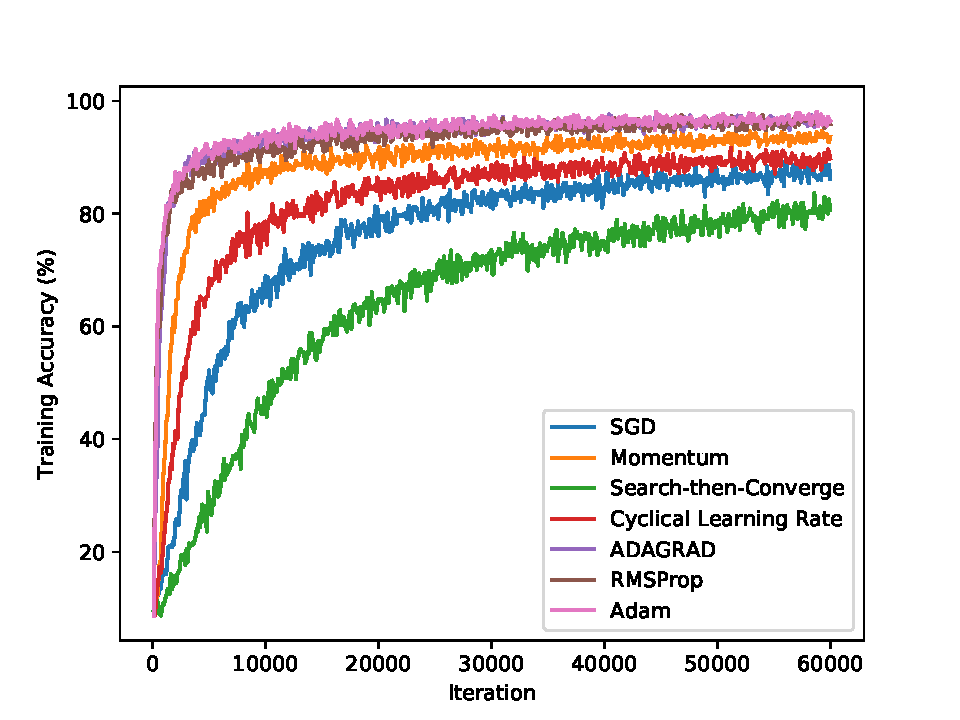
\includegraphics[width=\textwidth, keepaspectratio]{TrainAccuracy.pdf}	
\caption{Training Accuracy versus Iteration}
\end{figure}

\subsection{Training Loss versus Iteration}
\begin{figure}[H]
	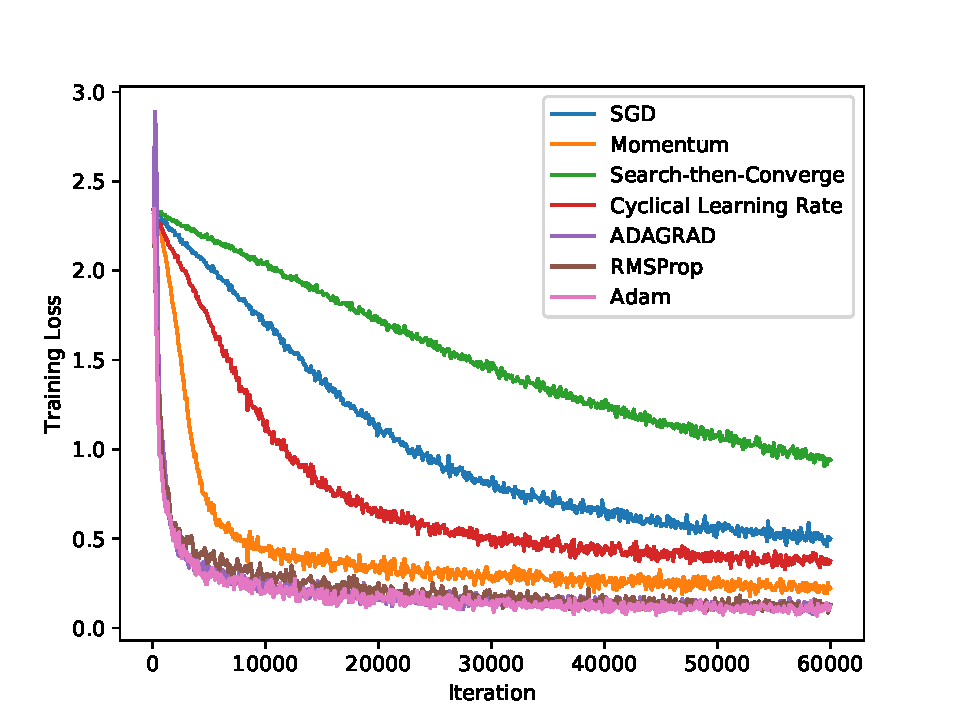
\includegraphics[width=\textwidth, keepaspectratio]{TrainLoss.pdf}	
	\caption{Training Loss versus Iteration}
\end{figure}

\subsection{Test Accuracy versus Iteration}
\subsubsection{Table}

	\begin{table}[H]
		\hskip-2.0cm\begin{tabular}{@{}|l|l|l|l|l|l|l|l|l|l|l|@{}}
			\toprule
			\multirow{2}{*}{Optimizer} & \multicolumn{10}{l|}{Iteration}                                              \\ \cmidrule(l){2-11} 
			& 6000 & 12000 & 18000 & 24000 & 30000 & 36000 & 42000 & 48000 & 54000 & 60000 \\ \midrule
			SGD                        & 58.3 & 72.8  & 78.3  & 81.8  & 83.9  & 85.3  & 86.2  & 87.0  & 87.6  & 88.1  \\ \midrule
			Momentum                   & 84.7 & 89.2  & 90.1  & 91.4  & 92.0  & 92.5  & 92.8  & 93.0  & 93.6  & 93.8  \\ \midrule
			Search-then-Converge       & 33.4 & 53.2  & 64.4  & 70.6  & 74.0  & 76.7  & 78.7  & 80.1  & 81.2  & 82.2  \\ \midrule
			Cyclical Learning Rate     & 71.6 & 80.9  & 84.7  & 86.7  & 87.8  & 88.6  & 89.2  & 89.7  & 90.0  & 90.4  \\ \midrule
			Adagrad                    & 91.4 & 93.7  & 94.4  & 95.2  & 95.6  & 95.9  & 96.1  & 96.4  &  96.6 & 96.6  \\ \midrule
			RMSProp                    & 88.8 & 92.4  & 93.5  & 94.7  & 94.9  & 95.5  & 95.9  & 96.1  & 96.4  & 96.5  \\ \midrule
			Adam                       & 92.1 & 94.1  & 94.8  & 95.5  & 96.0  & 96.4  & 96.6  & 96.6  & 96.7  & 96.9  \\ \bottomrule
		\end{tabular}
	
	\captionof{table}{Test Accuracy versus Iteration Matrix}
	\end{table}
	

\subsubsection{Plot}
\begin{figure}[H]
	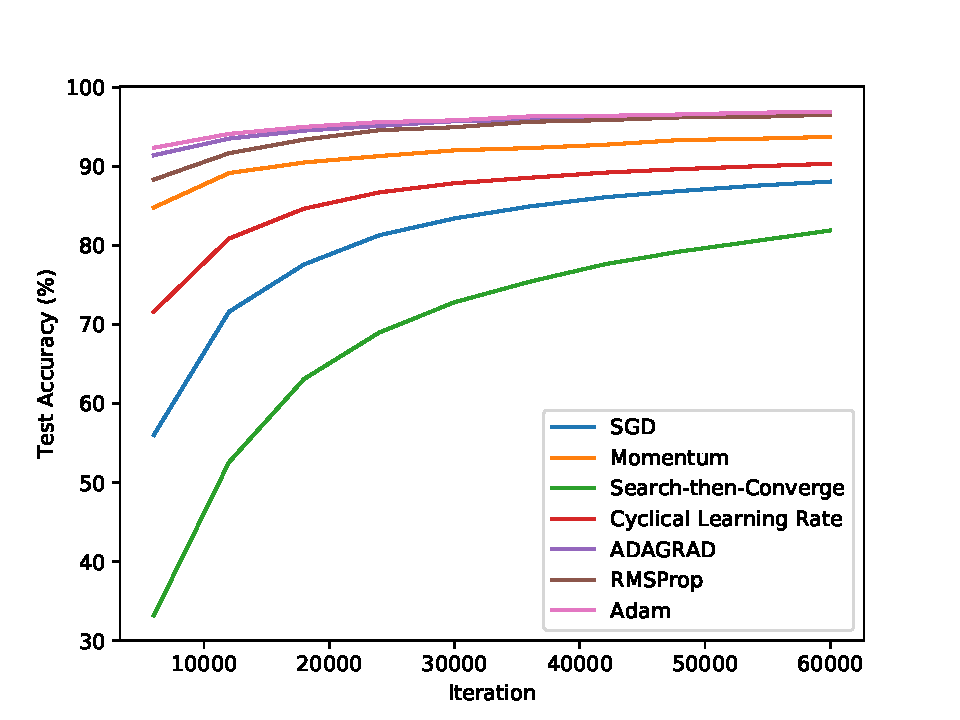
\includegraphics[width=\textwidth, keepaspectratio]{TestAcc.pdf}
	\caption{Test Accuracy versus Iteration}
\end{figure}
\subsection{Test Loss versus Iteration}
\subsubsection{Table}

	\begin{table}[H]
		\hskip-2.0cm\begin{tabular}{@{}|l|l|l|l|l|l|l|l|l|l|l|@{}}
			\toprule
			\multirow{2}{*}{Optimizer} & \multicolumn{10}{l|}{Iteration}                                              \\ \cmidrule(l){2-11} 
			& 6000 & 12000 & 18000 & 24000 & 30000 & 36000 & 42000 & 48000 & 54000 & 60000 \\ \midrule
			SGD                        & 1.94 & 1.55  & 1.18  & 0.92  & 0.77  & 0.66  & 0.59  & 0.53  & 0.50  & 0.47  \\ \midrule
			Momentum                   & 0.55 & 0.38  & 0.34  & 0.30  & 0.28  & 0.26  & 0.25  & 0.24  & 0.22  & 0.21  \\ \midrule
			Search-then-Converge       & 2.13 & 1.94  & 1.75  & 1.57  & 1.41  & 1.27  & 1.15  & 1.05  & 0.96  & 0.89  \\ \midrule
			Cyclical Learning Rate     & 1.60 & 0.96  & 0.68  & 0.55  & 0.48  & 0.44  & 0.41  & 0.38  & 0.37  & 0.35  \\ \midrule
			Adagrad                    & 0.28 & 0.21  & 0.18  & 0.15  & 0.14  & 0.13  & 0.13  & 0.12  & 0.11  & 0.11  \\ \midrule
			RMSProp                    & 0.37 & 0.25  & 0.21  & 0.17  & 0.16  & 0.14  & 0.14  & 0.12  & 0.11  & 0.11  \\ \midrule
			Adam                       & 0.26 & 0.19  & 0.16  & 0.14  & 0.13  & 0.12  & 0.11  & 0.11  & 0.10  & 0.09  \\ \bottomrule
		\end{tabular}
	
	
	\captionof{table}{Test Loss versus Iteration Matrix}	
	\end{table}

\subsubsection{Plot}
\begin{figure}[H]
	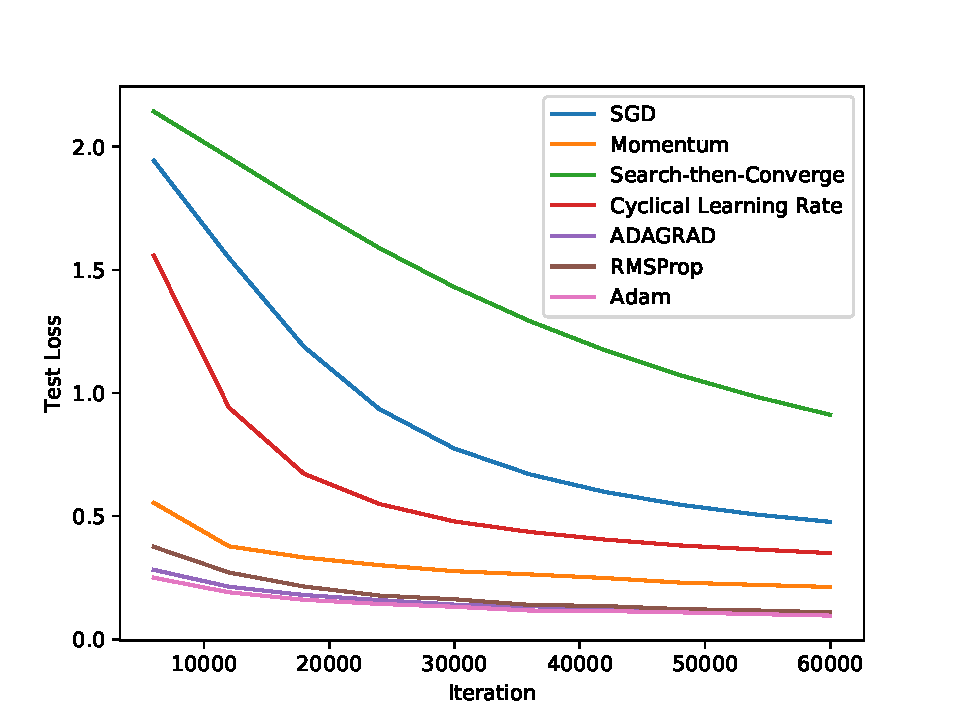
\includegraphics[width=\textwidth, keepaspectratio]{TestLoss.pdf}
	\setlength{\belowcaptionskip}{0.0pt}	
	\caption{Test Loss versus Iteration}
\end{figure}

\section{Analysis of results}
\subsection{Momentum}
This Optimizer performed the best amongst all of the non-adaptive learning rate Optimizers. This simplicity of this Optimizer is interesting to note as the simplest modification to SGD resulted in a large performance boost when compared to the slightly more convoluted CLR and STC Optimizers.

\subsection{Search-then-Converge} 
This was the only Optimizer that failed to perform better than SGD along our metrics. This is potentially due to a poor selection of the hyperparameter T. It seems the learning rate decayed too quickly which resulted in worse performance. However, with no well-defined best practice method for choosing T and receiving poor performance using the most intuitive approach to selecting T, retroactively increasing T to increase performance on our test set would go against the philosophy of having separate training and test sets.

\subsection{Cyclical Learning Rates}
This Optimizer performed better than SGD along all performance metrics as expected. It is important to note the lack of a precise method for choosing the hyperparameters of this Optimizer and future work should be put in to formalizing this selection method which could potentially increase the performance of this Optimizer in future.

\subsection{ADAGRAD}
This Optimizer was the second best performing Optimizer. This is interesting to note as it learns faster than RMSProp despite Adagrads monotonically decreasing learning rate. This suggests that the local minimum was quickly found and the decreasing learning rate aided the Optimizer in settling at the local minimum. This is supported by the fact that the gradient of the Test Accuracy Plot for Adagrad is low for the majority of the training process. 

\subsection{RMSProp}
This Optimizer performs worse than Adagrad earlier in the training epoch. However it converges to very similar performance to Adagrad and Adam at the end of the epoch. This suggests that RMSProp is not the best adaptive gradient optimizer for smaller datasets. However, for larger datasets the choice of adaptive gradient optimizer is mostly inconsequential. 

\subsection{Adam}

This Optimizer performed the best amongst all Optimizers. This corroborates the current body of research. It is interesting to note that the difference in performance between Adam and the other Adaptive gradient Optimizers is small considering the complexity of the Optimizer when compared to Adagrad and RMSProp. However, for real world applications where peak performance is required and minuscule differences in accuracy can result in excessive consequences, Adam should always be chosen amongst the Optimizers tested in this work. 
 


\section{Conclusion}
Selecting and understanding an Optimizer for Neural Networks can be difficult considering the level of mathematical and statistical knowledge required to understand each optimizer as well as the sheer variety of optimizers available. This paper sought to elucidate the differences between and compare the performance of Gradient-Descent-based Optimizers to aid the reader in understanding and choosing an Optimizer for their specific application. The Optimizers were compared on the MNIST dataset of handwritten digits and the training accuracy, test accuracy, training loss and test loss were compared with respect to the iteration count. The differences between each Optimizer were explained both theoretically and empirically thus achieving the purpose of this work.This work can be expanded upon in future by introducing new Optimizers for comparison as well as evaluation on different datasets or perhaps different Artificial Neural Network Architectures. 


\section{References}	
	
\bibliographystyle{plainnat}
\bibliography{mybib}

\end{document}







